\documentclass{standalone}
\usepackage[english]{babel}
% https://tex.stackexchange.com/questions/570303/use-blacktriangleright-as-itemize-label
\usepackage{amssymb} % for black triangleright

\renewcommand{\labelitemi}{$\textcolor{SwitchColor}{\bullet}$}
\renewcommand{\labelitemii}{$\textcolor{SwitchColor}{\blacktriangleright}$}
\renewcommand{\labelitemiii}{$\textcolor{SwitchColor}{\blacksquare}$}

% https://tex.stackexchange.com/questions/525959/prevent-latex-from-stretching-math
\setlength{\thinmuskip}{1\thinmuskip}
\setlength{\medmuskip}{1\medmuskip}
\setlength{\thickmuskip}{1\thickmuskip}

\usepackage{csquotes}
\usepackage{xcolor}
% \usepackage{anyfontsize}
\usepackage[export]{adjustbox}
% \usepackage[]{enumitem}
\usepackage{nicematrix}
\usepackage{tikz}
\usetikzlibrary{arrows.meta,positioning}
\usetikzlibrary{graphs}
\usetikzlibrary{patterns}
\usetikzlibrary{shadings}
\usetikzlibrary{mindmap, shadows, backgrounds} % , calc

\definecolor{SecondaryColor}{HTML}{BBAF01}
\definecolor{SecondaryColorDimmed}{HTML}{FEF684}
\definecolor{PrimaryColor}{HTML}{E95112}
\definecolor{PrimaryColorDimmed}{HTML}{F6AF91}
\colorlet{BoxColor}{gray!10!white}

% colored bold
% \newcommand\alert[1]{\textcolor{SwitchColor}{\textbf{#1}}}
\newcommand\alert[1]{\textcolor{SwitchColor}{#1}}

\newlength{\leveldistance}
\setlength{\leveldistance}{25cm}

\begin{document}
  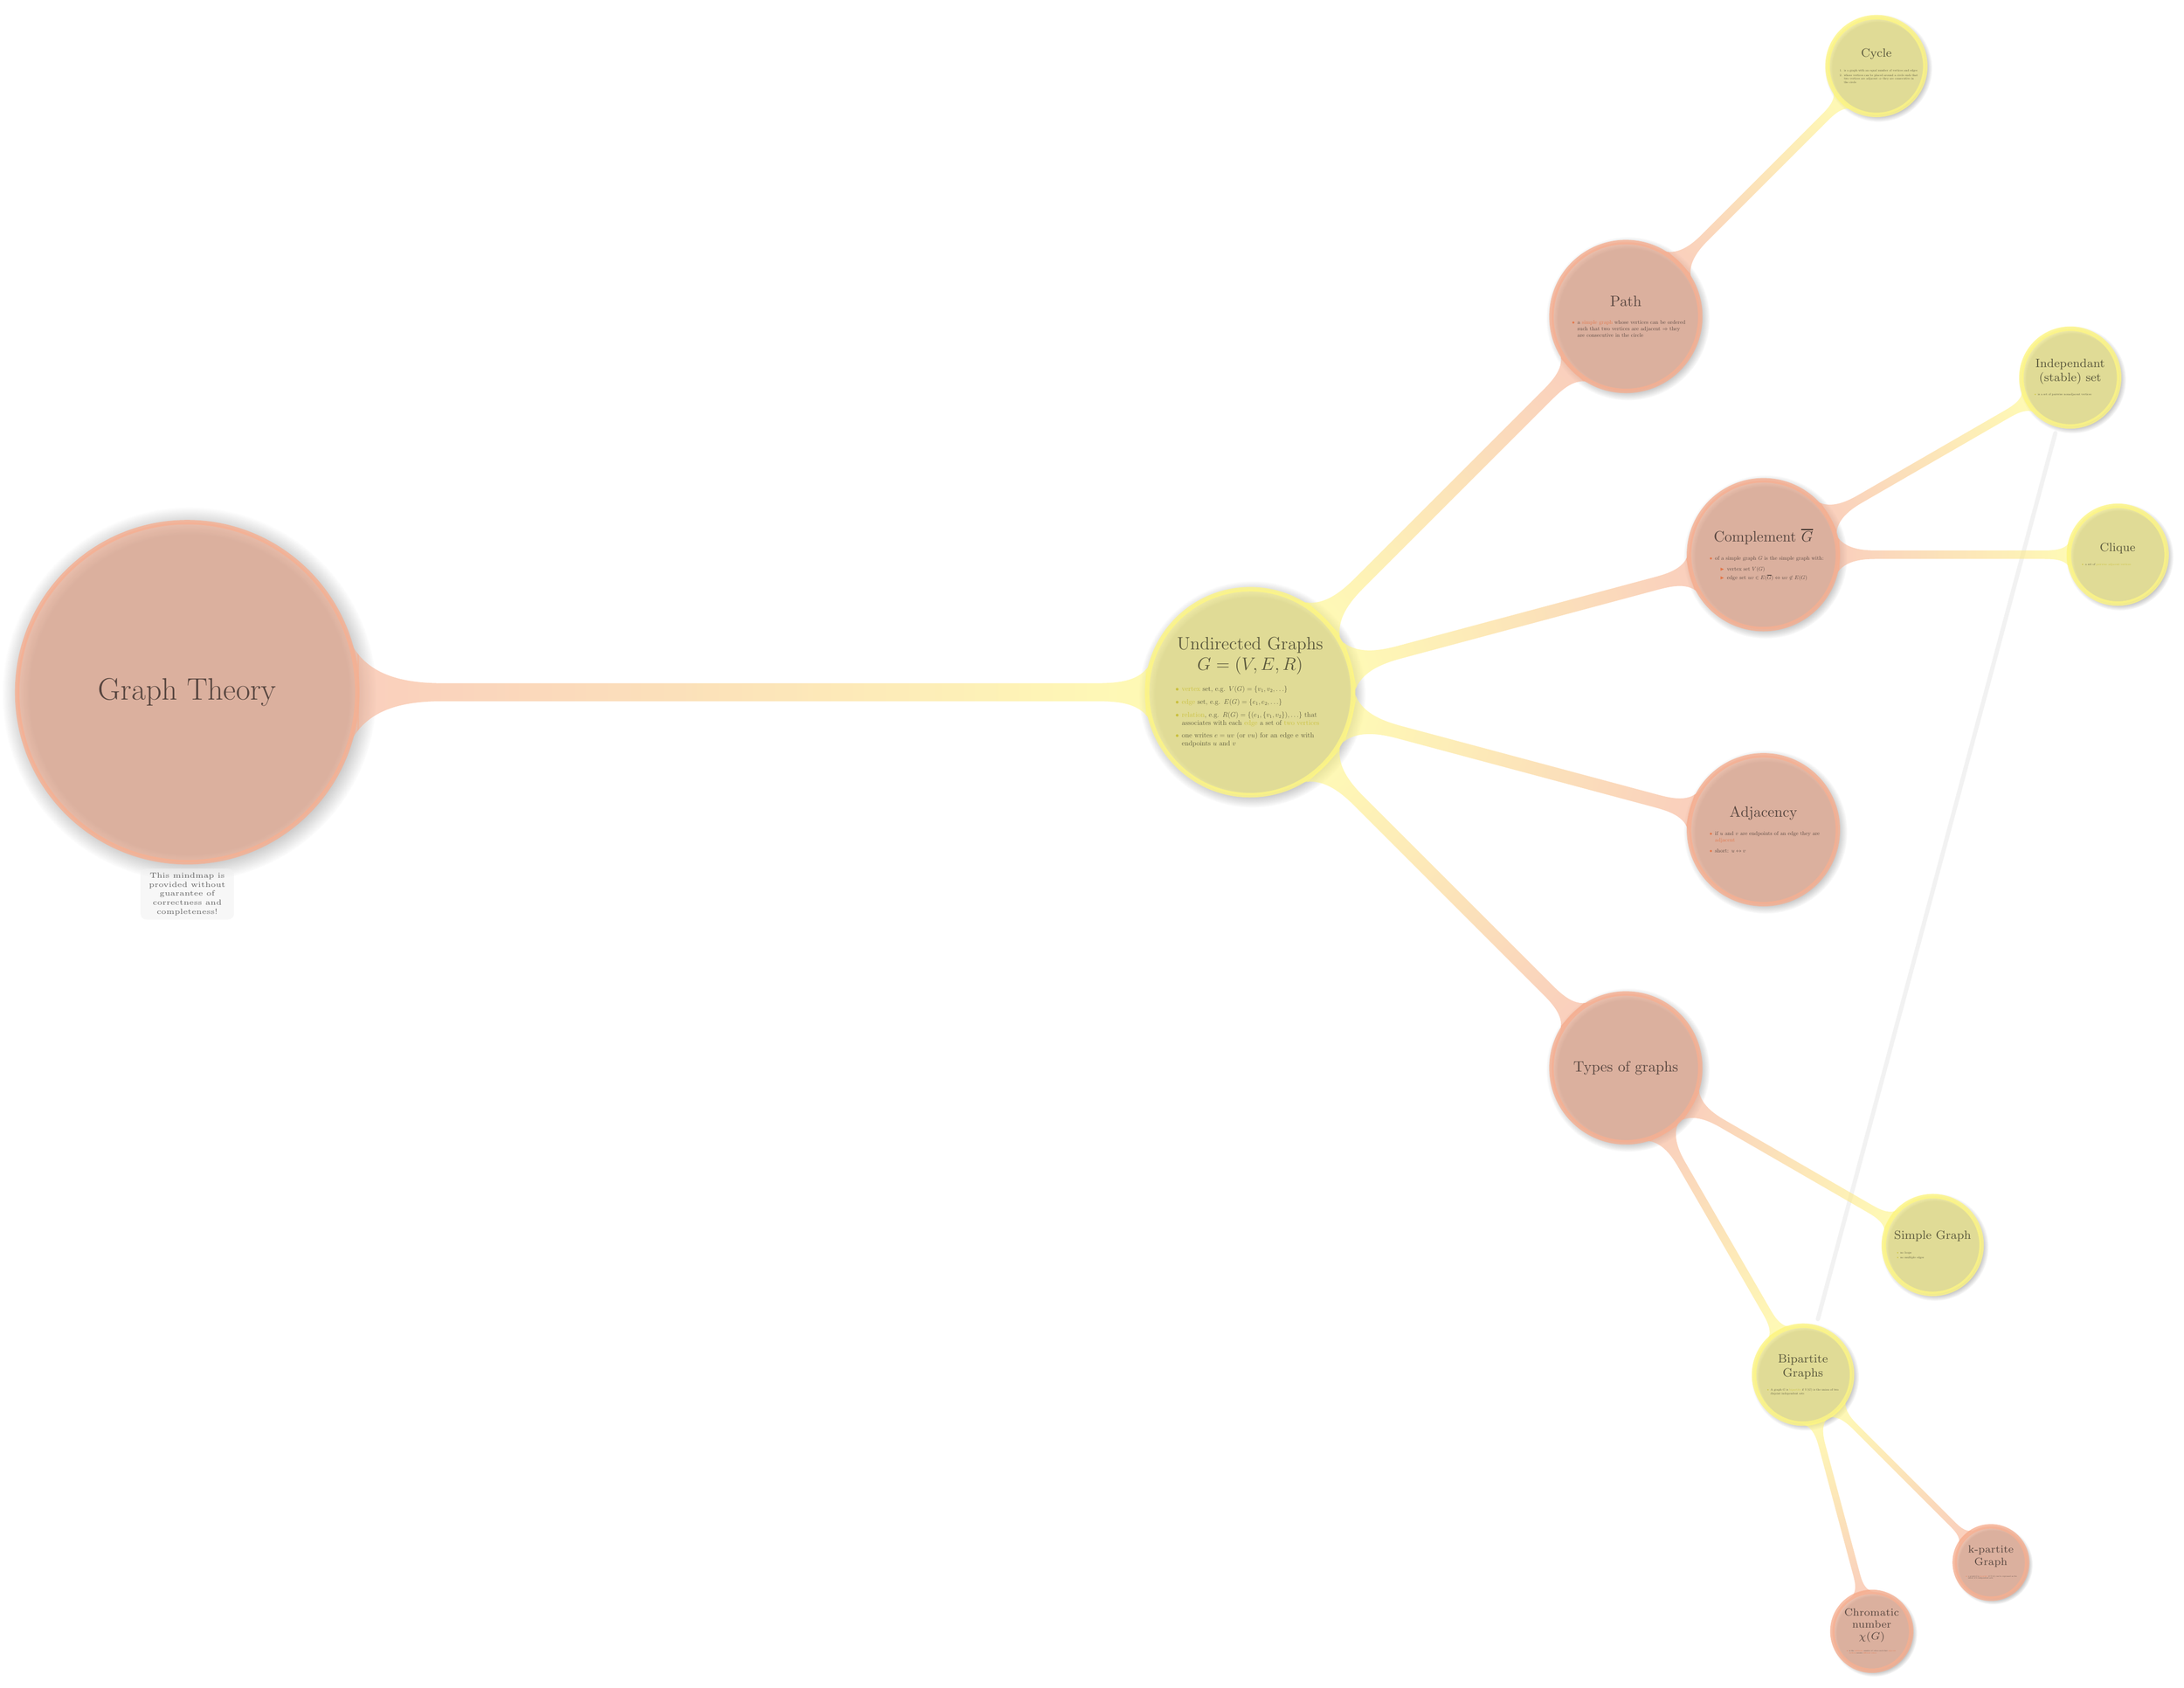
\begin{tikzpicture}[
      auto,
      huge mindmap,
      fill opacity=0.6,
      draw opacity=0.8,
      concept color = PrimaryColorDimmed,
      every annotation/.style={fill=BoxColor, draw=none, align=center, fill = BoxColor, text width = 2cm},
      grow cyclic,
      level 1/.append style = {
        concept color=SecondaryColorDimmed,
        level distance=\leveldistance,
        sibling angle=360/\the\tikznumberofchildren,
        % https://tex.stackexchange.com/questions/501240/trying-to-use-the-array-environment-inside-a-tikz-node-with-execute-at-begin-no
        execute at begin node=\definecolor{SwitchColor}{named}{SecondaryColor},
      },
      level 2/.append style = {
        concept color=PrimaryColorDimmed,
        level distance=\leveldistance / 2,
        sibling angle=30,
        execute at begin node=\definecolor{SwitchColor}{named}{PrimaryColor},
      },
      level 3/.append style = {
        concept color=SecondaryColorDimmed,
        level distance=\leveldistance / 3,
        execute at begin node=\definecolor{SwitchColor}{named}{SecondaryColor},
      },
      level 4/.append style = {
        concept color=PrimaryColorDimmed,
        level distance=\leveldistance / 4,
        execute at begin node=\definecolor{SwitchColor}{named}{PrimaryColor},
      },
      level 5/.append style = {
        concept color=SecondaryColorDimmed,
        level distance=\leveldistance / 5,
        execute at begin node=\definecolor{SwitchColor}{named}{SecondaryColor},
      },
      level 6/.append style = {
        concept color=PrimaryColorDimmed,
        level distance=\leveldistance / 6,
        execute at begin node=\definecolor{SwitchColor}{named}{PrimaryColor},
      },
      level 7/.append style = {
        concept color=SecondaryColorDimmed,
        level distance=\leveldistance / 7,
        execute at begin node=\definecolor{SwitchColor}{named}{SecondaryColor},
      },
      level 8/.append style = {
        concept color=PrimaryColorDimmed,
        level distance=\leveldistance / 8,
        execute at begin node=\definecolor{SwitchColor}{named}{PrimaryColor},
      },
      concept connection/.append style = {
        color = BoxColor,
      },
  ]
  % damit Annotationen nicht auch eine Drop Shadow erhalten
  \begin{scope}[
      every node/.style = {concept, circular drop shadow}, % draw=none
      every child/.style={concept},
    ]
  \node (gt) at (current page.center) {Graph Theory}
  child {
    node {Undirected Graphs $G = (V, E, R)$
      \resizebox{\textwidth}{!}{
        \begin{minipage}[t]{10cm}
          \begin{itemize}
            \item \alert{vertex} set, e.g. $V(G) = \{v_1, v_2, \ldots\}$
            \item \alert{edge} set, e.g. $E(G) = \{e_1, e_2, \ldots\}$
            \item \alert{relation}, e.g. $R(G) = \{(e_1, \{v_1, v_2\}), \ldots\}$ that associates with each \alert{edge} a set of \alert{two vertices}
            \item one writes $e = uv$ (or $vu$) for an edge e with endpoints $u$ and $v$
          \end{itemize}
        \end{minipage}
      }
    }
      child {
        node {Types of graphs}
          child {
            node (bipartite graphs) {Bipartite Graphs
              \resizebox{\textwidth}{!}{
                \begin{minipage}[t]{8cm}
                  \begin{itemize}
                    \item A graph $G$ is \alert{bipartite} if $V(G)$ is the union of two disjoint independent sets
                  \end{itemize}
                \end{minipage}
              }
            }
            child {
              node {Chromatic number $\chi(G)$
                \resizebox{\textwidth}{!}{
                  \begin{minipage}[t]{8cm}
                    \begin{itemize}
                      \item is the \alert{minimum} number of colors such that \alert{adjacent vertices} receive \alert{different colors}
                    \end{itemize}
                  \end{minipage}
                }
              }
            }
            child {
              node {k-partite Graph
                \resizebox{\textwidth}{!}{
                  \begin{minipage}[t]{8cm}
                    \begin{itemize}
                      \item a graph $G$ is \alert{k-partite} if $V(G)$ can be expressed as the union of $k$ independent sets
                    \end{itemize}
                  \end{minipage}
                }
              }
            }
          }
          child {
            node (simple graph) {Simple Graph
              \resizebox{\textwidth}{!}{
                \begin{minipage}[t]{8cm}
                  \begin{itemize}
                    \item no loops
                    \item no multiple edges
                  \end{itemize}
                \end{minipage}
              }
            }
          }
      }
      child {
        node {Adjacency
          \resizebox{\textwidth}{!}{
            \begin{minipage}[t]{8cm}
              \begin{itemize}
                \item if $u$ and $v$ are endpoints of an edge they are \alert{adjacent}
                \item short: $u\leftrightarrow v$
              \end{itemize}
            \end{minipage}
          }
        }
      }
      child {
        % https://latex.org/forum/viewtopic.php?t=8650
        node {Complement $\overline{G}$
          \resizebox{\textwidth}{!}{
            \begin{minipage}[t]{8cm}
            \begin{itemize}
              \item of a simple graph $G$ is the simple graph with:
              \begin{itemize}
                \item vertex set $V(G)$
                \item edge set $uv \in E(\overline{G}) \Leftrightarrow uv\not\in E(G)$
              \end{itemize}
            \end{itemize}
            \end{minipage}
          }
        }
          child {
            node {Clique
              \resizebox{\textwidth}{!}{
                \begin{minipage}[t]{8cm}
                  \begin{itemize}
                    \item a set of \alert{pairwise adjacent vertices}
                  \end{itemize}
                \end{minipage}
              }
            }
          }
          child {
            node (independant set) {Independant (stable) set
              \resizebox{\textwidth}{!}{
                \begin{minipage}[t]{8cm}
                  \begin{itemize}
                    \item is a set of pairwise nonadjacent vertices
                  \end{itemize}
                \end{minipage}
              }
            }
          }
      }
      child {
        node {Path
          \resizebox{\textwidth}{!}{
            \begin{minipage}[t]{8cm}
              \begin{itemize}
                \item a \alert{simple graph} whose vertices can be ordered such that two vertices are adjacent $\Rightarrow$ they are consecutive in the circle
              \end{itemize}
            \end{minipage}
          }
        }
          child {
            node {Cycle
              \resizebox{\textwidth}{!}{
                \begin{minipage}[t]{8cm}
                  \begin{enumerate}
                    \item is a graph with an equal number of vertices and edges
                    \item whose vertices can be placed around a circle such that two vertices are adjacent $\Rightarrow$ they are consecutive in the circle
                  \end{enumerate}
                \end{minipage}
              }
            }
          }
      }
    };
  \end{scope}
  % ┌───────────────────┐
  % │ Verbindungslinien │
  % └───────────────────┘
  \begin{pgfonlayer}{background}
    \draw [concept connection]
  %     (commoncasefast) edge (amdahl)
  %     (branchpredictionbuffer) edge (2bitpredictor)
  %     (loadusedatahazard) edge (forwarding)
      (bipartite graphs) edge (independant set);
  \end{pgfonlayer}
  % ┌──────────────┐
  % │ Annotationen │
  % └──────────────┘
  % https://tex.stackexchange.com/questions/302976/node-positioning-middle-point-mind-map-connection-bar
  \node [annotation, below] at (gt.south) {This mindmap is provided without guarantee of correctness and completeness!};
  % \path (measuringexecutiontime) -- node[annotation, above, align=center, pos=0.01] {Similiar to \textbf{Response Time:} How long it takes to do a task} (ca);
  % \path (performance) -- node[annotation, above, align=center, pos=0.01] {Similiar to \textbf{Throughput}: Total work done per time unit (e.g. tasks, transactions\ldots / per hour)} (ca);
  % \path (elapsedtime) -- node[annotation, above, align=center, pos=0.01] {Also called \textbf{Wall Clock Time} or \textbf{Real Time}} (ca);
  % \path (cputime) -- node[annotation, above, align=center, pos=0.01] {Also called \textbf{User Time}} (ca);
  % % \path (branchpredictionbuffer) -- node[annotation, below, align=center, pos=-0.06] {Also called Branch History Table} (ca);
  % \path (multicycle) -- node[annotation, above, align=center, pos=0.01] {Optimize space} (ca);
  % \path (pipelining) -- node[annotation, above, align=center, pos=0.01] {Optimize time} (ca);
  \end{tikzpicture}
\end{document}
